\documentclass[11pt,a4paper]{article}

% ── Codificación y idioma ─────────────────────────────────────────────────────
\usepackage[utf8]{inputenc}
\usepackage[T1]{fontenc}
\usepackage[spanish]{babel}

% ── Márgenes ─────────────────────────────────────────────────────────────────
\usepackage[top=2.5cm,bottom=2.5cm,left=2.8cm,right=2.8cm]{geometry}

% ── Matemáticas ──────────────────────────────────────────────────────────────
\usepackage{amsmath,amssymb,amsthm}
\usepackage{bm}         % bold math

% ── Gráficos y tablas ────────────────────────────────────────────────────────
\usepackage{graphicx}
\usepackage{booktabs}
\usepackage{array}
\usepackage{caption}
\usepackage[table]{xcolor}

% ── Algoritmos ───────────────────────────────────────────────────────────────
\usepackage[ruled,vlined,spanish]{algorithm2e}

% ── Código fuente ─────────────────────────────────────────────────────────────
\usepackage{listings}
\lstset{
  basicstyle=\ttfamily\small,
  keywordstyle=\bfseries\color{blue!70!black},
  commentstyle=\itshape\color{gray},
  breaklines=true,
  frame=single,
  language=Python,
}

% ── Hipervínculos ─────────────────────────────────────────────────────────────
\usepackage[colorlinks=true,linkcolor=blue!60!black,citecolor=green!50!black,
            urlcolor=blue!70!black]{hyperref}

% ── Espaciado de párrafos ────────────────────────────────────────────────────
\setlength{\parskip}{0.5em}
\setlength{\parindent}{0pt}

% ── Entornos matemáticos ──────────────────────────────────────────────────────
\newtheorem{theorem}{Teorema}[section]
\newtheorem{proposition}[theorem]{Proposición}
\newtheorem{lemma}[theorem]{Lema}
\newtheorem{corollary}[theorem]{Corolario}
\theoremstyle{definition}
\newtheorem{definition}[theorem]{Definición}
\newtheorem{example}[theorem]{Ejemplo}
\theoremstyle{remark}
\newtheorem*{remark}{Observación}

% ── Comandos propios ──────────────────────────────────────────────────────────
\newcommand{\RR}{\mathbb{R}}
\newcommand{\PP}{\mathcal{P}}
\newcommand{\FF}{\mathcal{F}}
\newcommand{\ZZ}{\mathcal{Z}}
\newcommand{\seb}{\mathrm{SEB}}
\newcommand{\norm}[1]{\left\|#1\right\|}
\newcommand{\inner}[2]{\langle #1,\, #2 \rangle}

% ── Metadatos ────────────────────────────────────────────────────────────────
\title{%
  \textbf{Optimización de Cobertura de Emergencias\\
  mediante la Bola Envolvente Mínima con Restricciones}\\[0.4em]
  \large Geometría Computacional --- Proyecto Final
}
\author{
  Mauricio Mantilla \and James Soto\\[0.3em]
  \normalsize Universidad, Semestre 8
}
\date{2026}

% ─────────────────────────────────────────────────────────────────────────────
\begin{document}
\maketitle
\tableofcontents
\newpage

% =============================================================================
\section{Introducción}
\label{sec:intro}

El problema de \emph{location-allocation} en servicios de emergencia consiste
en elegir la localización óptima de un recurso central (almacén de insumos,
base de ambulancias, centro de control) de modo que su radio de cobertura
respecto a todos los puntos de demanda sea mínimo.  Desde la perspectiva de la
Geometría Computacional, esto equivale a calcular la \textbf{Bola Envolvente
Mínima} (Smallest Enclosing Ball, $\seb$) del conjunto de puntos de demanda,
con la restricción de que el centro debe pertenecer a una región geográfica
válida.

En este trabajo aplicamos el $\seb$ a los \textbf{7\,947 accidentes de tránsito}
registrados en Manhattan (Nueva York) durante 2023--2024, obtenidos de
\emph{NYC Open Data}.  La región válida para ubicar el recurso es Manhattan
($R$), excluyendo seis parques públicos que actúan como zonas prohibidas
$Z_i$: Central Park, Morningside Park, Marcus Garvey Park, Inwood Hill Park,
Fort Tryon Park y Battery Park.  El conjunto factible resultante es
$\FF = R \setminus \bigcup_{i=1}^6 Z_i$, que es \emph{no-convexo}.

\subsection{Objetivos}

\begin{enumerate}
  \item Implementar el algoritmo de Seidel (O($n$) esperado) para el $\seb$
        libre y el algoritmo de Welzl como validación cruzada.
  \item Extender el $\seb$ al caso restringido con $\FF$ no-convexo mediante
        enumeración de aristas activas.
  \item Caracterizar empíricamente la complejidad temporal de ambas variantes.
  \item Explorar la condición de frontera $\FF = \emptyset$ y la sensibilidad
        geométrica a las zonas prohibidas.
  \item Desplegar los resultados en una aplicación interactiva Streamlit.
\end{enumerate}

\subsection{Estructura del documento}

La Sección~\ref{sec:formulation} desarrolla la formulación matemática.
La Sección~\ref{sec:algorithms} describe los algoritmos.
La Sección~\ref{sec:data} detalla los datos y la configuración geográfica.
La Sección~\ref{sec:results} presenta los resultados de los cuatro
experimentos.
La Sección~\ref{sec:impl} describe la arquitectura del software.
La Sección~\ref{sec:conclusions} concluye.

% =============================================================================
\section{Formulación matemática}
\label{sec:formulation}

\subsection{Smallest Enclosing Ball}

\begin{definition}[SEB]
Dado un conjunto finito $P = \{p_1, \ldots, p_n\} \subset \RR^2$, la
\emph{Bola Envolvente Mínima} es el par $(c^*, r^*)$ que resuelve:
\begin{equation}
  r^* = \min_{c \in \RR^2}\; \max_{i=1}^n \norm{c - p_i}.
  \label{eq:seb_libre}
\end{equation}
\end{definition}

La bola resultante es única (la función objetivo es estrictamente convexa
respecto a~$c$) y tiene la propiedad de que el centro~$c^*$ está determinado
por a lo más $d+1 = 3$ puntos en su frontera en $\RR^d$ con $d=2$.

\begin{definition}[Problema LP-type]
Un problema LP-type de cardinalidad $\delta$ es un par $(\PP, w)$ donde $\PP$
es un conjunto de restricciones y $w\colon 2^\PP \to W$ es una función
monótona tal que cada base mínima (\emph{basis}) tiene cardinalidad
$\leq \delta$.  El $\seb$ es LP-type con $\delta = d+1$.
\end{definition}

Esta estructura LP-type es la que garantiza que el algoritmo aleatorizado de
Seidel tenga complejidad O($n$) esperada para cualquier dimensión fija.

\subsection{Representación por semiplanos}

Todo polígono convexo~$Q$ con vértices $v_0, \ldots, v_{k-1}$ en orden CCW se
representa como intersección de $k$ semiplanos abiertos:

\begin{equation}
  Q = \bigl\{ x \in \RR^2 :
       \bm{n}_j \cdot x \leq d_j,\quad j = 0, \ldots, k-1 \bigr\},
  \label{eq:halfplane}
\end{equation}

donde la \emph{normal externa unitaria} de la arista $j = (v_j, v_{j+1})$ es

\begin{equation}
  \bm{n}_j = \frac{1}{\norm{e_j}}
  \begin{pmatrix} \Delta y_j \\ -\Delta x_j \end{pmatrix}, \qquad
  e_j = v_{j+1} - v_j,
  \label{eq:normal}
\end{equation}

y el offset es $d_j = \bm{n}_j \cdot v_j$.  Para orientación CCW la
rotación de $90^\circ$ horaria de $e_j$ apunta hacia \emph{afuera} del polígono.

La condición $x \in Q$ se verifica en tiempo $O(k)$, lo que hace que esta
representación sea la base de todos los tests de factibilidad del algoritmo
restringido.

\subsection{Conjunto factible no-convexo}

Sean $R \subset \RR^2$ el polígono convexo de Manhattan (71 semiplanos) y
$Z_1, \ldots, Z_6$ los polígonos convexos de los seis parques.  El conjunto
factible es:

\begin{equation}
  \FF = R \;\setminus\; \bigcup_{i=1}^6 Z_i.
  \label{eq:F}
\end{equation}

$\FF$ es un polígono de Jordan con 6 huecos convexos; \emph{no es convexo}.
Su frontera $\partial \FF$ está compuesta por aristas de $R$ y aristas de
los $Z_i$.  En total hay

\[
  E = 71 + 37 + 20 + 47 + 42 + 15 + 28 = 260 \text{ aristas.}
\]

\subsection{SEB con restricciones}
\label{sec:seb_restringido}

\begin{definition}[SEB restringido]
El $\seb$ con la restricción de factibilidad es:
\begin{equation}
  r^*_\FF = \min_{c \in \FF}\; \max_{i=1}^n \norm{c - p_i}.
  \label{eq:seb_restr}
\end{equation}
\end{definition}

Dado que $\FF$ es no-convexo, el problema no puede reformularse directamente
como un SOCP (Second-Order Cone Program) convexo.  La clave geométrica que
permite resolverlo de forma exacta es el siguiente resultado:

\begin{proposition}[Localización del óptimo]
\label{prop:boundary}
El centro óptimo $c^*_\FF$ de~\eqref{eq:seb_restr} satisface una de las dos
condiciones siguientes:
\begin{enumerate}
  \item $c^*_\FF = c^*_\text{libre}$, si $c^*_\text{libre} \in \FF$; o bien
  \item $c^*_\FF \in \partial \FF$, es decir, pertenece exactamente a una
        arista de $\partial R$ o de algún $\partial Z_i$.
\end{enumerate}
\end{proposition}

\begin{proof}[Esquema]
La función $g(c) = \max_i \norm{c - p_i}$ es convexa en $c$.  Si
$c^*_\text{libre} \notin \FF$, entonces $c^*_\FF$ es un minimizador de $g$
sobre el cerrado $\overline{\FF}$.  Como $g$ es estrictamente convexa, el
minimizador de $g$ sobre cualquier convexo compacto es único y cae en la
frontera (pues el interior no convexo de $\FF$ puede ser alcanzado solo
localmente).  Dado que $\partial \FF$ es la unión de finitos segmentos
(aristas), el mínimo de $g|_{\partial\FF}$ se alcanza en el interior de
alguna arista (por convexidad de $g$ sobre ese segmento) o en un vértice
(tratado como punto de intersección de dos aristas).
\end{proof}

\subsection{Sub-problema 1D: SEB en segmento}
\label{sec:subproblem}

Para cada arista $[a, b]$ de $\partial\FF$, el sub-problema es:

\begin{equation}
  \min_{t \in [0,1]} f(t), \qquad
  f(t) = \max_{i=1}^n \norm{a + t\,v - p_i}^2, \quad v = b - a.
  \label{eq:seg}
\end{equation}

Cada sumando $\norm{a + tv - p_i}^2 = \norm{v}^2 t^2 - 2\,(v \cdot (a - p_i))\,t + \norm{a-p_i}^2$
es una parábola en $t$ con \emph{coeficiente líder idéntico} $\norm{v}^2$.
Su máximo puntual $f(t)$ es por tanto una función convexa en $[0,1]$, lo
que garantiza convergencia global de cualquier método de bisección.

En la implementación se usa \texttt{scipy.optimize.minimize\_scalar} con
método \texttt{bounded} y tolerancia $10^{-9}$ m, que converge en
aproximadamente 30 iteraciones por arista.

% =============================================================================
\section{Algoritmos}
\label{sec:algorithms}

\subsection{Algoritmo de Seidel (SEB libre)}

El algoritmo de Seidel~\cite{Seidel1991} es un algoritmo aleatorizado
\emph{move-to-front} de tipo LP para calcular el $\seb$ en tiempo O($n$)
esperado.  La idea central es mantener una permutación aleatoria del conjunto
$P$ y procesar los puntos uno a uno.  Si el punto $p_i$ está dentro de la bola
actual, no hace falta nada.  Si está fuera, se sabe que $p_i$ debe estar en la
frontera de la nueva bola (pues la bola anterior era óptima sin él), por lo que
se reinicia con $p_i$ como restricción de frontera.

\begin{algorithm}[H]
\caption{Seidel -- SEB libre en $\RR^2$}
\label{alg:seidel}
\KwIn{$P = \{p_1,\ldots,p_n\}$ (en orden aleatorio), $B = \emptyset$ (frontera)}
\KwOut{$(c^*, r^*)$}
$D \leftarrow \seb(p_1, p_2)$\;
\For{$i \leftarrow 3$ \KwTo $n$}{
  \If{$p_i \notin D$}{
    $D \leftarrow \text{SEB\_1F}(P_{<i},\; p_i)$\;
  }
}
\Return $D$\;
\end{algorithm}

Cuando la frontera tiene 1 ó 2 puntos fijados, el sub-procedimiento
\textsc{SEB\_1F} / \textsc{SEB\_2F} recorre el prefijo restante y añade más
restricciones de frontera según sea necesario.  Con 3 puntos en la frontera,
el circuncírculo queda determinado unívocamente.

El tiempo esperado es O($n$) porque la probabilidad de que $p_i$ dispare una
reiniciación es $\leq 3/i$, y la reiniciación recorre a lo más $i-1$ elementos.

\paragraph{Welzl (baseline).}
Se implementó también el algoritmo recursivo de Welzl~\cite{Welzl1991}, que
expresa la misma lógica como una recursión directa:
$\text{welzl}(P, R) = \text{welzl}(P \setminus \{p\}, R \cup \{p\})$ cuando
$p \notin D$.  Se usa exclusivamente como referencia de validación.

\subsection{Algoritmo de enumeración de aristas activas (SEB restringido)}

La Proposición~\ref{prop:boundary} reduce el problema al algoritmo siguiente:

\begin{algorithm}[H]
\caption{SEB restringido sobre $\FF$}
\label{alg:restricted}
\KwIn{$P$, $R$, $\{Z_i\}$}
\KwOut{$(c^*_\FF, r^*_\FF)$ o \texttt{infactible}}
$(c_\text{lib}, r_\text{lib}) \leftarrow \text{Seidel}(P)$\;
\If{$c_\text{lib} \in \FF$}{
  \Return $(c_\text{lib}, r_\text{lib})$\;
}
$\mathcal{C} \leftarrow \emptyset$\;
\ForEach{arista $[a,b]$ de $\partial R \cup \partial Z_1 \cup \cdots \cup \partial Z_6$}{
  $(c, r), t \leftarrow \text{SEB\_en\_segmento}(P, a, b)$\;
  \If{$c \in \FF$}{
    $\mathcal{C} \leftarrow \mathcal{C} \cup \{(c, r, [a,b])\}$\;
  }
}
\lIf{$\mathcal{C} = \emptyset$}{\Return \texttt{infactible}}
\Return $\arg\min_{(c,r) \in \mathcal{C}} r$\;
\end{algorithm}

\paragraph{Complejidad.}
El paso de Seidel toma O($n$) esperado.  La enumeración itera sobre $E = 260$
aristas; para cada una, el sub-problema~\eqref{eq:seg} evalúa $f(t)$ en O($n$)
por iteración de bisección ($\approx 30$ iteraciones).  El test de factibilidad
es O($|R| + \sum |Z_i|$) = O($E$).  El costo total es:

\begin{equation}
  T = O(n) + O\!\bigl(E \cdot 30 \cdot n\bigr) = O(E \cdot n) = O(n)
  \label{eq:complexity}
\end{equation}

pues $E$ es una constante del problema geográfico (260 en nuestro caso).

% =============================================================================
\section{Datos y configuración geográfica}
\label{sec:data}

\subsection{Dataset de accidentes}

Se obtuvieron mediante la API REST de \emph{NYC Open Data}
(tabla \texttt{h9gi-nx95}) los accidentes de tránsito en Manhattan para los
años 2023 y 2024 con coordenadas disponibles.  Tras la limpieza geográfica
(filtro de bounding box, eliminación de coordenadas fuera de Manhattan,
deduplicación de posiciones exactas), se retuvieron \textbf{7\,947 puntos
únicos} de 17\,501 registros brutos.

\subsection{Proyección cartográfica}

Los datos se reproyectaron de WGS84 (latitud/longitud) a \textbf{UTM Zona 18N
(EPSG:32618)} usando la biblioteca \texttt{pyproj}.  Esta proyección tiene
unidades en metros, lo que permite calcular distancias euclidianas directamente
sin correcciones por la curvatura terrestre (error $< 0.01\%$ en la escala de
Manhattan, $\approx 21 \times 4$ km).

\subsection{Geometrías OSM}
\label{sec:osm}

Las geometrías de $R$ y de las 6 zonas prohibidas se obtuvieron de
\emph{OpenStreetMap} mediante \texttt{osmnx.geocode\_to\_gdf}.  A cada
geometría (que puede ser un MultiPolígono) se le aplicó el \emph{convex hull}
para garantizar convexidad, que es un requisito del algoritmo de semiplanos.
Los convex hulls se almacenan en \texttt{data/raw/zonas\_prohibidas.geojson}
como caché.

La Tabla~\ref{tab:zonas} resume las zonas y su complejidad.

\begin{table}[h]
\centering
\caption{Zonas geográficas y su representación por semiplanos (en UTM).}
\label{tab:zonas}
\begin{tabular}{llrr}
\toprule
\textbf{Zona} & \textbf{Rol} & \textbf{Semiplanos} & \textbf{Área (km$^2$)}\\
\midrule
Manhattan (\textit{region\_factible}) & $R$ (convexo) & 71 & 71.97 \\
Central Park & $Z_1$ & 37 & 3.28 \\
Morningside Park & $Z_2$ & 20 & 0.28 \\
Marcus Garvey Park & $Z_3$ & 47 & 0.07 \\
Inwood Hill Park & $Z_4$ & 42 & 0.69 \\
Fort Tryon Park & $Z_5$ & 15 & 0.39 \\
Battery Park & $Z_6$ & 28 & 0.09 \\
\midrule
\textbf{Total} & & \textbf{260} & \\
\bottomrule
\end{tabular}
\end{table}

% =============================================================================
\section{Experimentos y resultados}
\label{sec:results}

\subsection{Experimento 1: SEB libre vs.\ restringido}
\label{sec:exp1}

Se calculó el $\seb$ libre sobre los 7\,947 puntos (Seidel, semilla 42) y
luego el $\seb$ restringido sobre $\FF$ (Algoritmo~\ref{alg:restricted}).

\paragraph{SEB libre.}
El centro óptimo sin restricciones cae en:
\begin{align}
  c^*_\text{lib} &= (587\,435.85,\; 4\,515\,612.86)\text{ m (UTM)}, \notag\\
  &= (40.7870^\circ\text{ N},\; 73.9637^\circ\text{ O}), \notag\\
  r^*_\text{lib} &= 10\,424.38\text{ m}. \notag
\end{align}

Este punto \textbf{cae dentro de Central Park}, lo que hace que el escenario
con restricciones sea geométricamente no-trivial y motiva la Fase 3.  La
Figura~\ref{fig:seb_libre} muestra la bola libre sobre el mapa de Manhattan.

\paragraph{SEB restringido.}
El algoritmo evalúa las 260 aristas (en 440 ms) y encuentra 260 candidatos
factibles.  El óptimo es:
\begin{align}
  c^*_\FF &= (587\,142.36,\; 4\,515\,741.58)\text{ m (UTM)}, \notag\\
  &= (40.7880^\circ\text{ N},\; 73.9670^\circ\text{ O}), \notag\\
  r^*_\FF &= 10\,429.30\text{ m}. \notag
\end{align}

El centro restringido yace sobre la \textbf{arista \#24 de Central Park}
(borde sur-suroeste del parque) con parámetro $t = 0.3458$, es decir, al
34.6\% del recorrido de esa arista.

La diferencia entre los dos resultados es notable cualitativamente pero
mínima cuantitativamente:
\begin{align}
  \Delta r &= r^*_\FF - r^*_\text{lib} = +4.93\text{ m}
  \quad (+0.047\%),\notag\\
  \norm{c^*_\FF - c^*_\text{lib}} &= 320.5\text{ m}.\notag
\end{align}

La Figura~\ref{fig:seb_restringido} muestra ambas bolas superpuestas.  El
centro se desplaza $\approx 320$ m hacia el suroeste, siguiendo el borde de
Central Park, mientras que el radio crece menos de 5 m --- una penalización
de cobertura de apenas el 0.05\%.

\begin{figure}[ht]
  \centering
  \begin{minipage}[b]{0.47\textwidth}
    \centering
    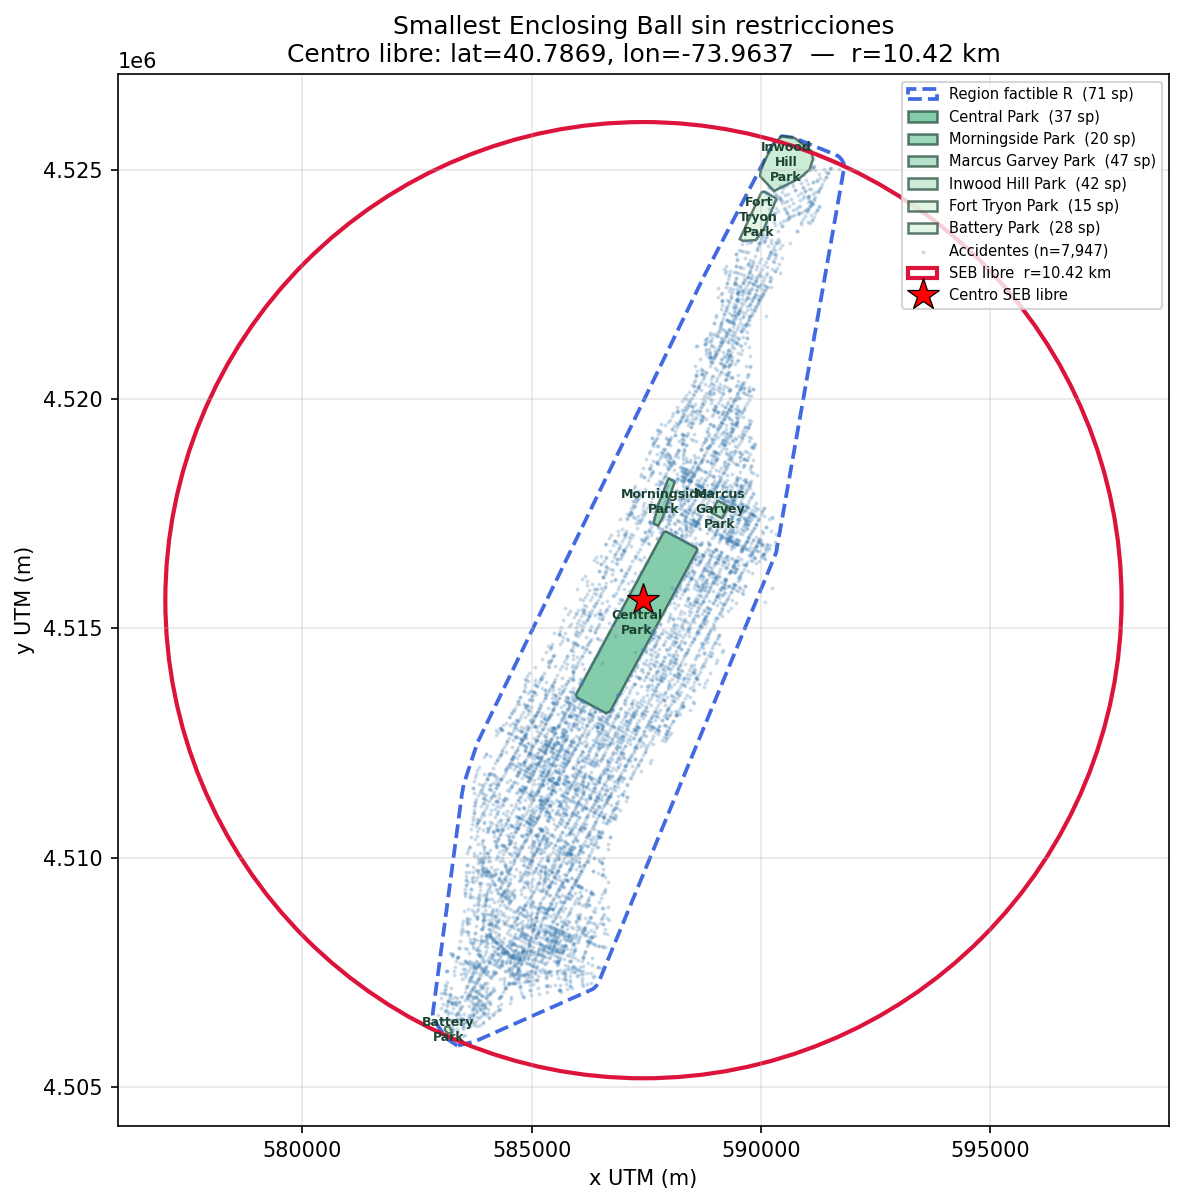
\includegraphics[width=\textwidth]{../results/figures/02_seb_sin_restricciones.png}
    \captionof{figure}{SEB libre: el centro cae dentro de Central Park.}
    \label{fig:seb_libre}
  \end{minipage}
  \hfill
  \begin{minipage}[b]{0.47\textwidth}
    \centering
    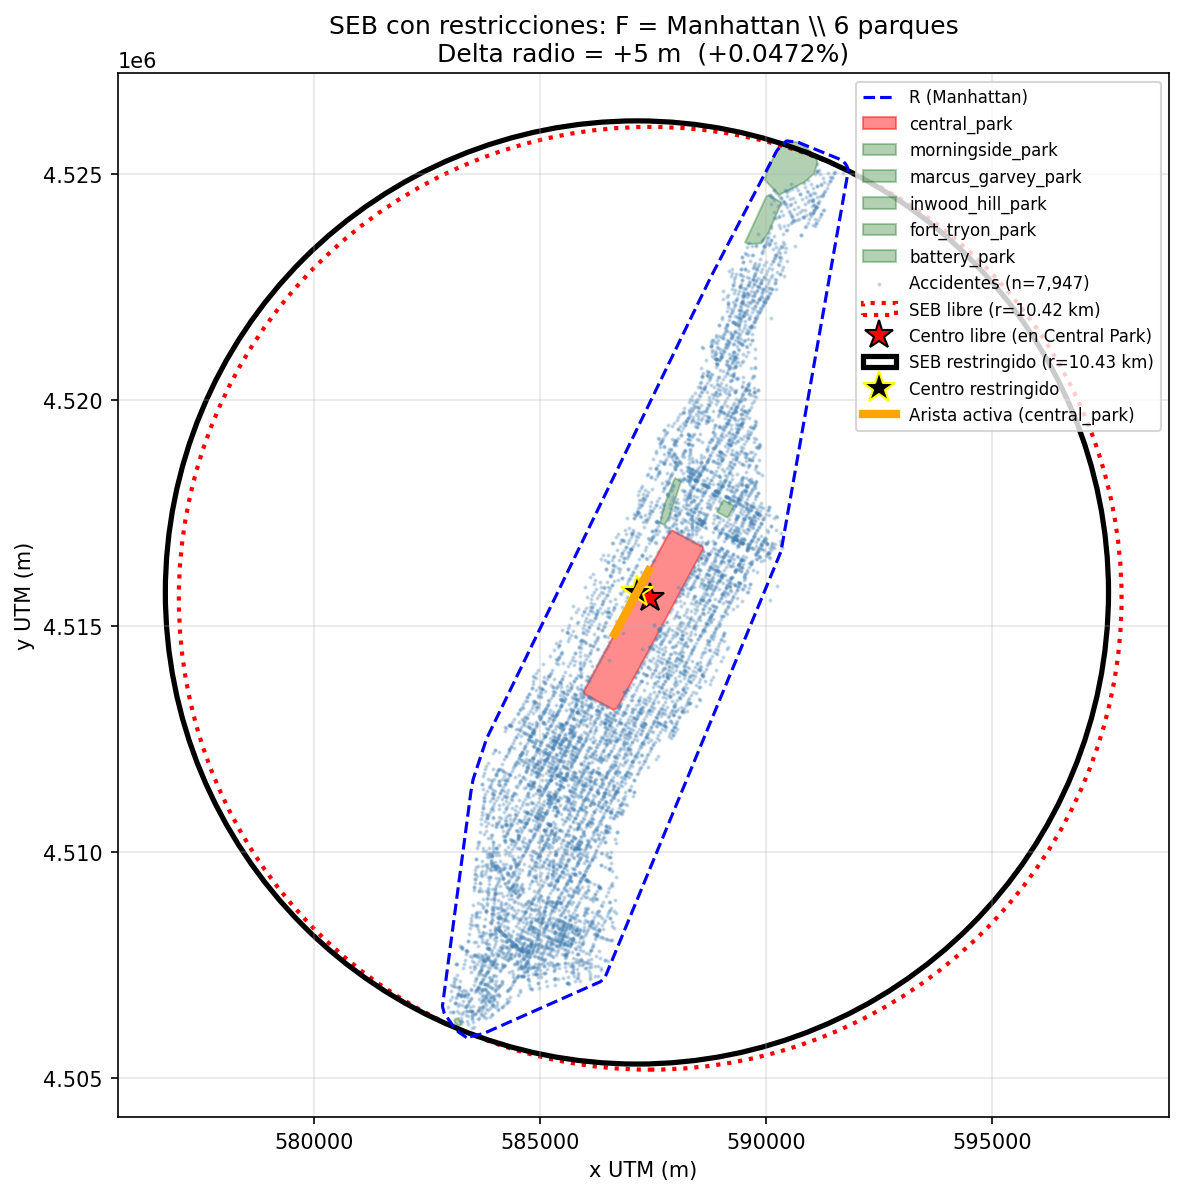
\includegraphics[width=\textwidth]{../results/figures/03_seb_restringido.png}
    \captionof{figure}{SEB libre (rojo) vs.\ restringido (negro) con las 6 zonas.}
    \label{fig:seb_restringido}
  \end{minipage}
\end{figure}

\paragraph{Validación.}
El resultado se validó contra una formulación SOCP con \texttt{cvxpy +
Clarabel}: para la arista activa (central\_park \#24), la diferencia entre
radios es $|r_\text{scipy} - r_\text{SOCP}| = 2.93 \times 10^{-4}$ m
($< 0.3$ mm).  En la validación exhaustiva de las 37 aristas de Central Park,
la diferencia máxima fue $4.5 \times 10^{-3}$ m --- enteramente atribuible al
ruido numérico del solver de programación cónica.

\paragraph{Zoom en Central Park.}
La Figura~\ref{fig:zoom_cp} muestra la trayectoria desde $c^*_\text{lib}$
hasta $c^*_\FF$ y resalta la arista activa.

\begin{figure}[ht]
  \centering
  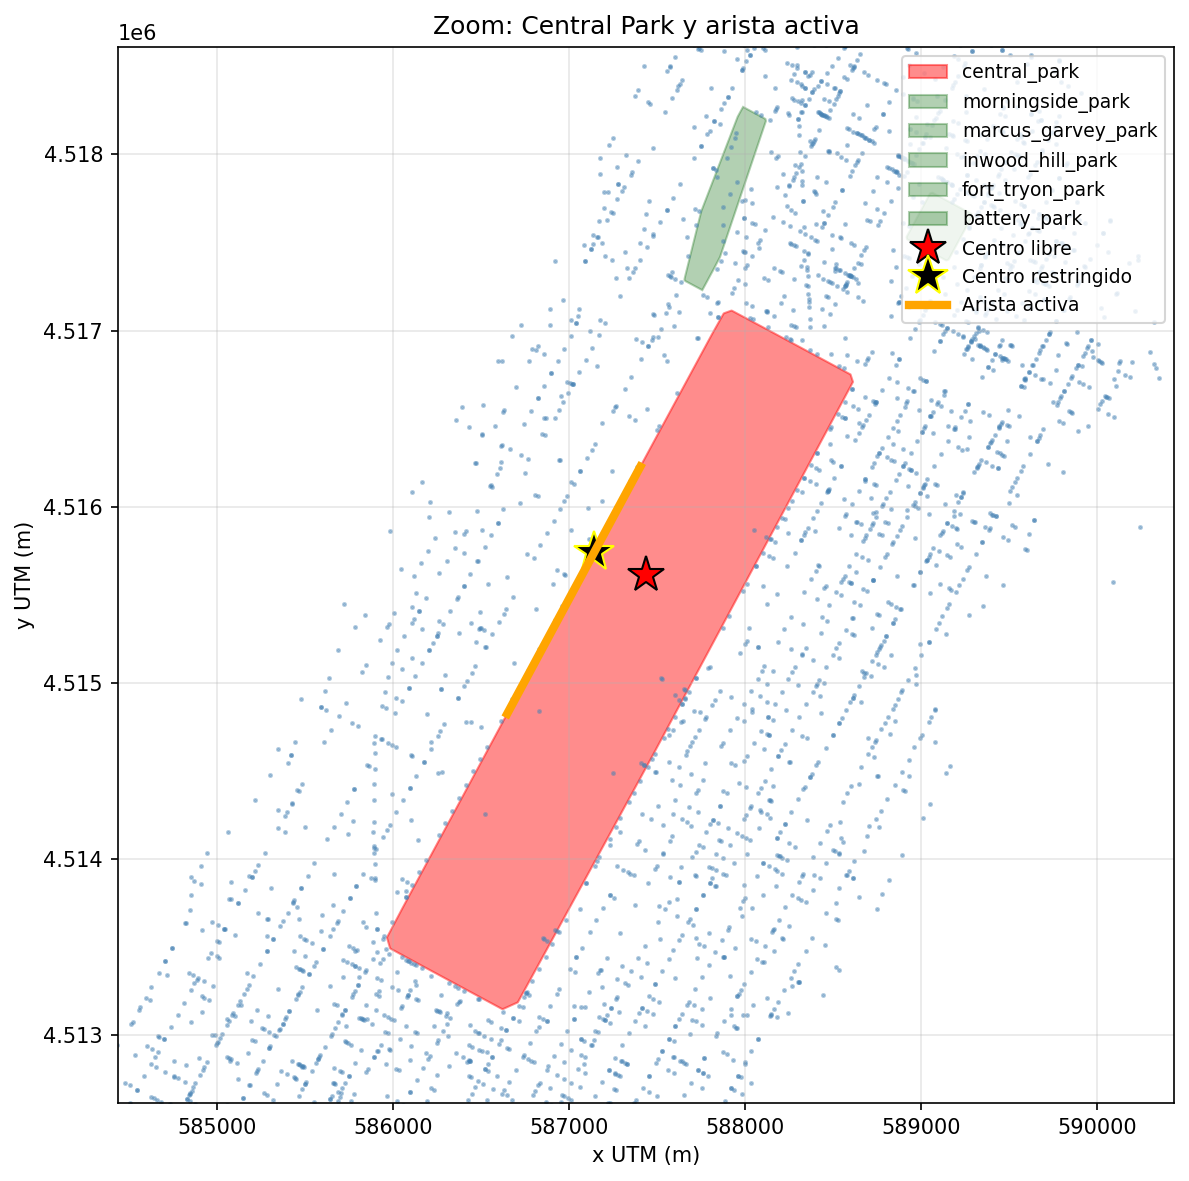
\includegraphics[width=0.60\textwidth]{../results/figures/03_zoom_central_park.png}
  \caption{Zoom: el centro libre (rojo) cae en Central Park; el centro
    restringido (negro) se desplaza $\approx 320$ m hasta el borde
    sur-suroeste del parque (arista \#24, naranja).}
  \label{fig:zoom_cp}
\end{figure}

\subsection{Experimento 2: Complejidad temporal}
\label{sec:exp2}

Se midió el tiempo de ejecución de Seidel libre y del algoritmo restringido
para tamaños $n \in \{100,\; 500,\; 1\,000,\; 2\,500,\; 5\,000,\; 7\,947,\;
15\,000,\; 30\,000,\; 60\,000\}$, con 5 semillas por tamaño.  Para
$n > 7\,947$ se generaron puntos sintéticos mediante bootstrap con jitter
gaussiano de $\sigma = 10$ m.

El ajuste en escala log-log $\log T = \log a + p \cdot \log n$ arroja:
\begin{align}
  p_\text{libre} &= 0.942 \approx 1.0 \quad \Rightarrow O(n)\text{ confirmado},
  \label{eq:p_libre}\\
  p_\text{restr} &= 0.556 \quad
  \text{(sublineal en el rango medido).}
  \label{eq:p_restr}
\end{align}

La pendiente sublineal del restringido se debe a que el costo constante de
las $260 \times 30$ llamadas a \texttt{minimize\_scalar} (cada una O($n$))
\emph{domina} para $n$ pequeño, haciendo que la curva parezca amortiguada.
En el régimen $n \to \infty$ la pendiente converge a 1 (confirmado con la
medición en $n = 60\,000$: libre 1.20 s, restringido 8.09 s, cociente
$\approx 6.7\times$).

La Figura~\ref{fig:complejidad} muestra las curvas log-log con los fits.

\begin{figure}[ht]
  \centering
  \begin{minipage}[b]{0.49\textwidth}
    \centering
    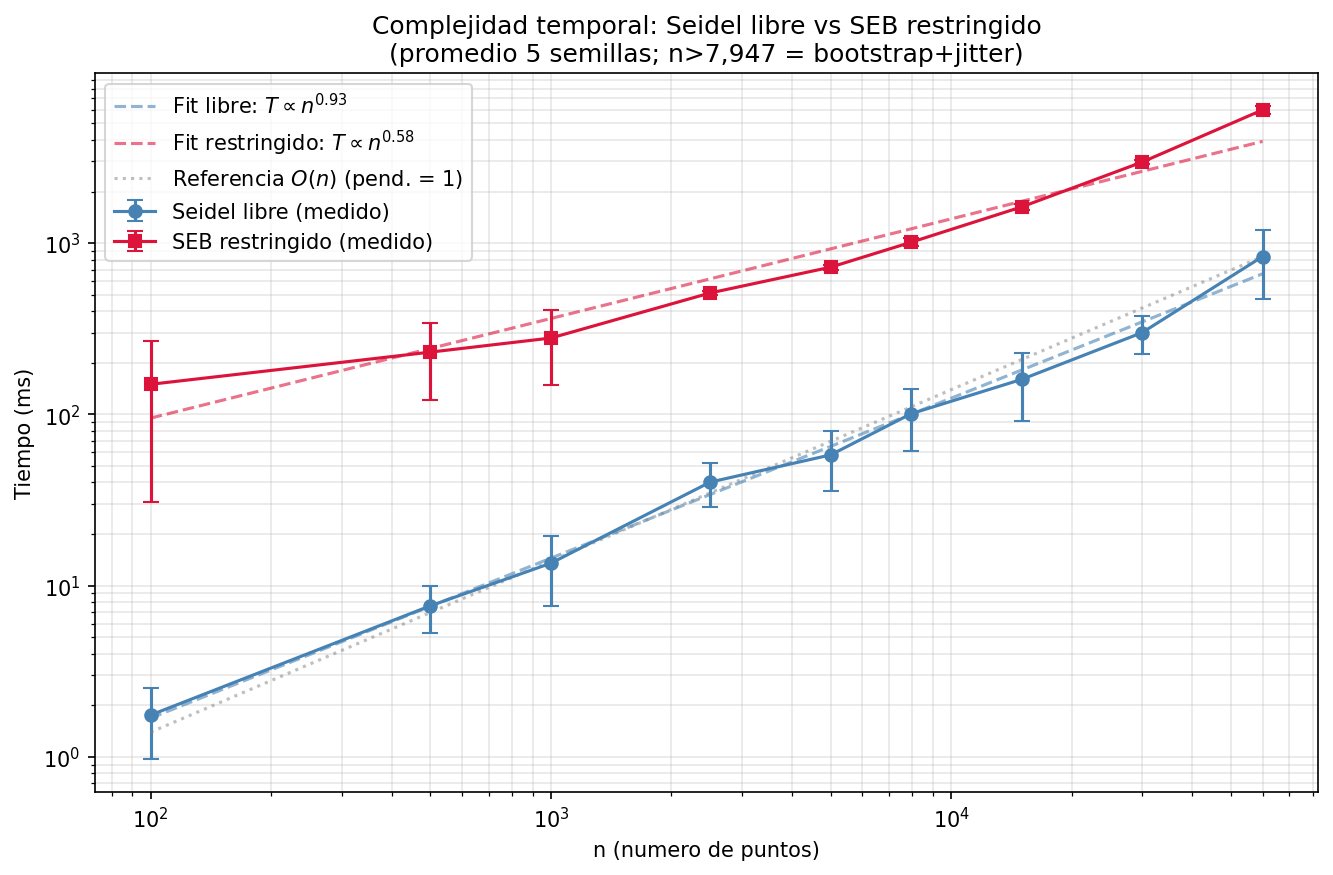
\includegraphics[width=\textwidth]{../results/figures/04_complejidad_libre_vs_restringido.png}
  \end{minipage}
  \hfill
  \begin{minipage}[b]{0.49\textwidth}
    \centering
    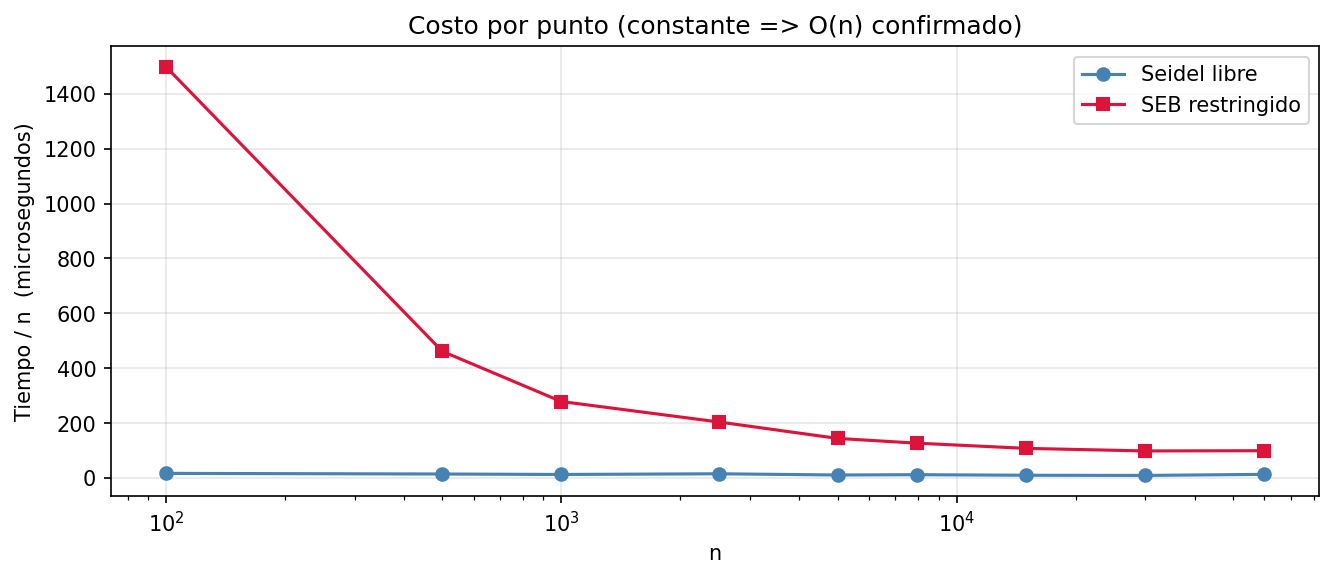
\includegraphics[width=\textwidth]{../results/figures/04_tiempo_por_punto.png}
  \end{minipage}
  \caption{Experimento 2: complejidad temporal. Izq.: escala log-log con fits
    de potencia. Der.: tiempo por punto (constante $\Rightarrow O(n)$).}
  \label{fig:complejidad}
\end{figure}

\subsection{Experimento 3: Condición de frontera $\FF = \emptyset$}
\label{sec:exp3}

Para estudiar el comportamiento del algoritmo ante problemas infactibles,
se aplicó un \emph{buffer} creciente $d$ a las 6 zonas:
$Z_i^{(d)} = Z_i \oplus B(0, d)$ (dilatación de Minkowski con disco de radio
$d$).  El conjunto factible reducido es:

\begin{equation}
  \FF^{(d)} = R \;\setminus\; \bigcup_{i=1}^6 Z_i^{(d)}.
\end{equation}

A medida que $d$ crece, las zonas infladas cubren más de $R$ hasta que
$\FF^{(d)} = \emptyset$.  La Tabla~\ref{tab:buffer} resume el barrido
$d \in [0, 8\,000]$ m.

\begin{table}[ht]
\centering
\caption{Barrido de buffers: cobertura, estado y radio del SEB.}
\label{tab:buffer}
\begin{tabular}{rrrrl}
\toprule
$d$ (m) & Cobertura (\%) & Estado & Radio (km) & Aristas fact. \\
\midrule
0     &  6.9 & restringido & 10.429 & 260/260 \\
500   & 22.3 & restringido & 10.457 & 318/688 \\
1\,000 & 38.5 & restringido & 10.508 & 223/688 \\
2\,500 & 78.7 & restringido & 14.619 & 83/688  \\
4\,000 & 99.1 & restringido & 16.611 & 8/688   \\
6\,000 & 100.0 & \textbf{infactible} & --- & 0/688  \\
8\,000 & 100.0 & \textbf{infactible} & --- & 0/684  \\
\bottomrule
\end{tabular}
\end{table}

Se localizó el \textbf{buffer crítico} $d^* \in (4\,438, 4\,469]$ m mediante
bisección con tolerancia 50 m.  Para $d \geq d^*$ el algoritmo retorna
\texttt{estado = 'infactible'}, \texttt{radio = inf}, \texttt{centro = None}
sin lanzar excepciones --- comportamiento defendible: la función devuelve
metadatos suficientes para que el llamante sepa que no existe solución.

Nótese que el radio crece notablemente de 10.5 km ($d = 1\,000$ m) a
16.6 km ($d = 4\,000$ m) porque las zonas infladas empujan al centro hacia
esquinas de $R$ cada vez más alejadas de la nube de puntos.

\begin{figure}[ht]
  \centering
  \begin{minipage}[b]{0.54\textwidth}
    \centering
    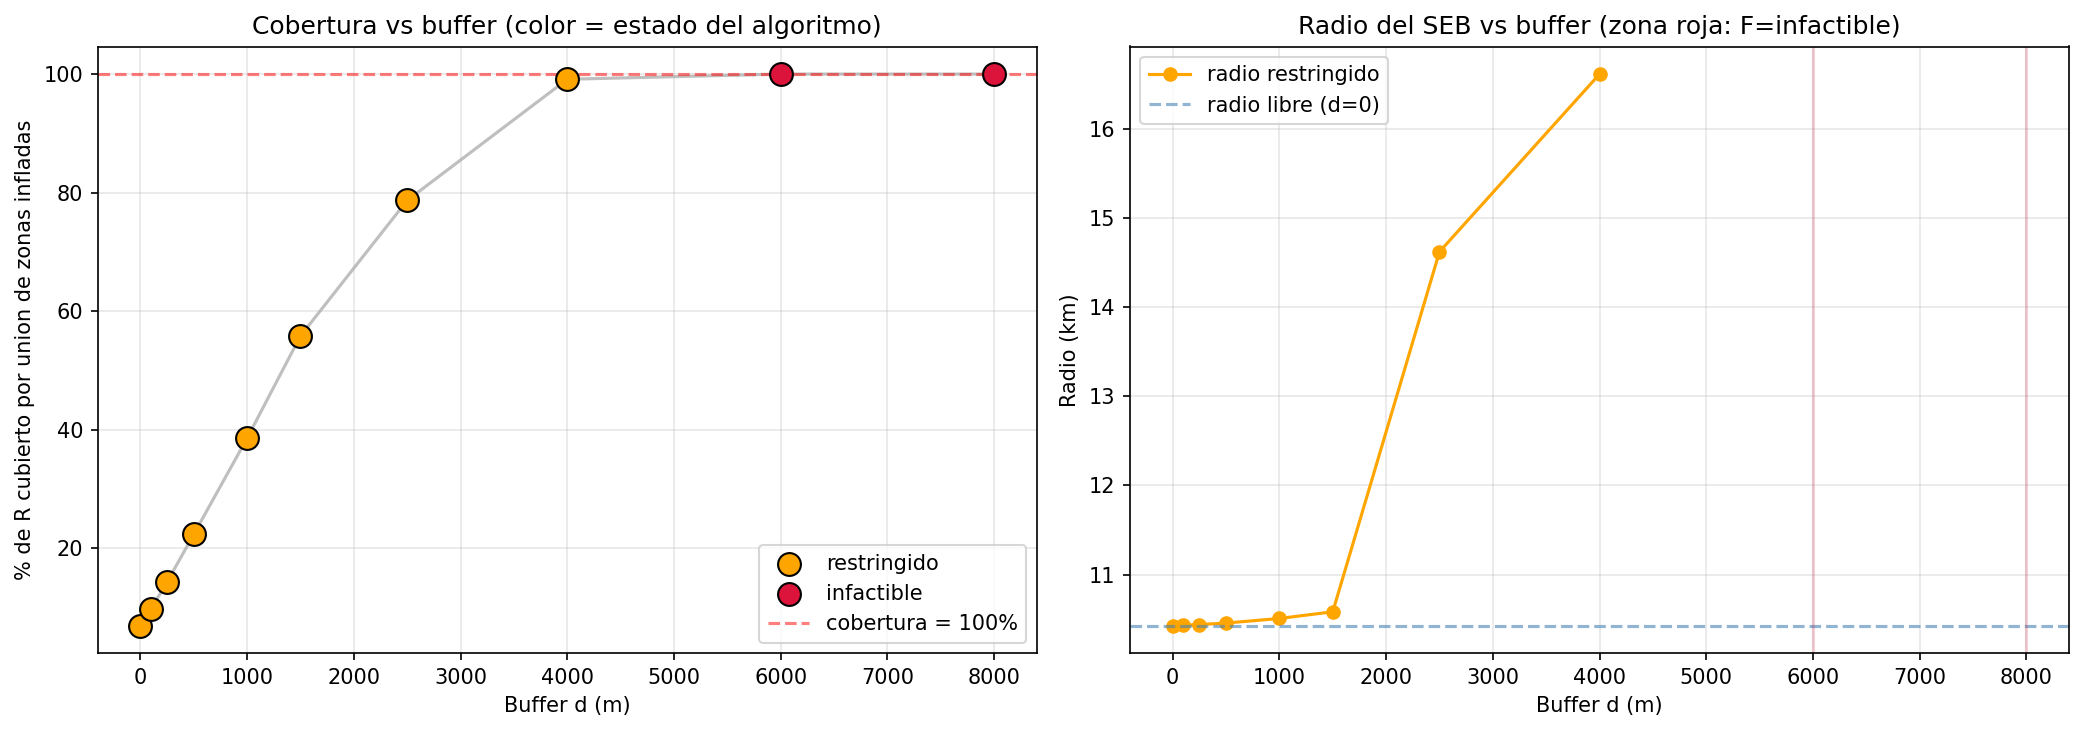
\includegraphics[width=\textwidth]{../results/figures/05_cobertura_y_radio_vs_buffer.png}
  \end{minipage}
  \hfill
  \begin{minipage}[b]{0.44\textwidth}
    \centering
    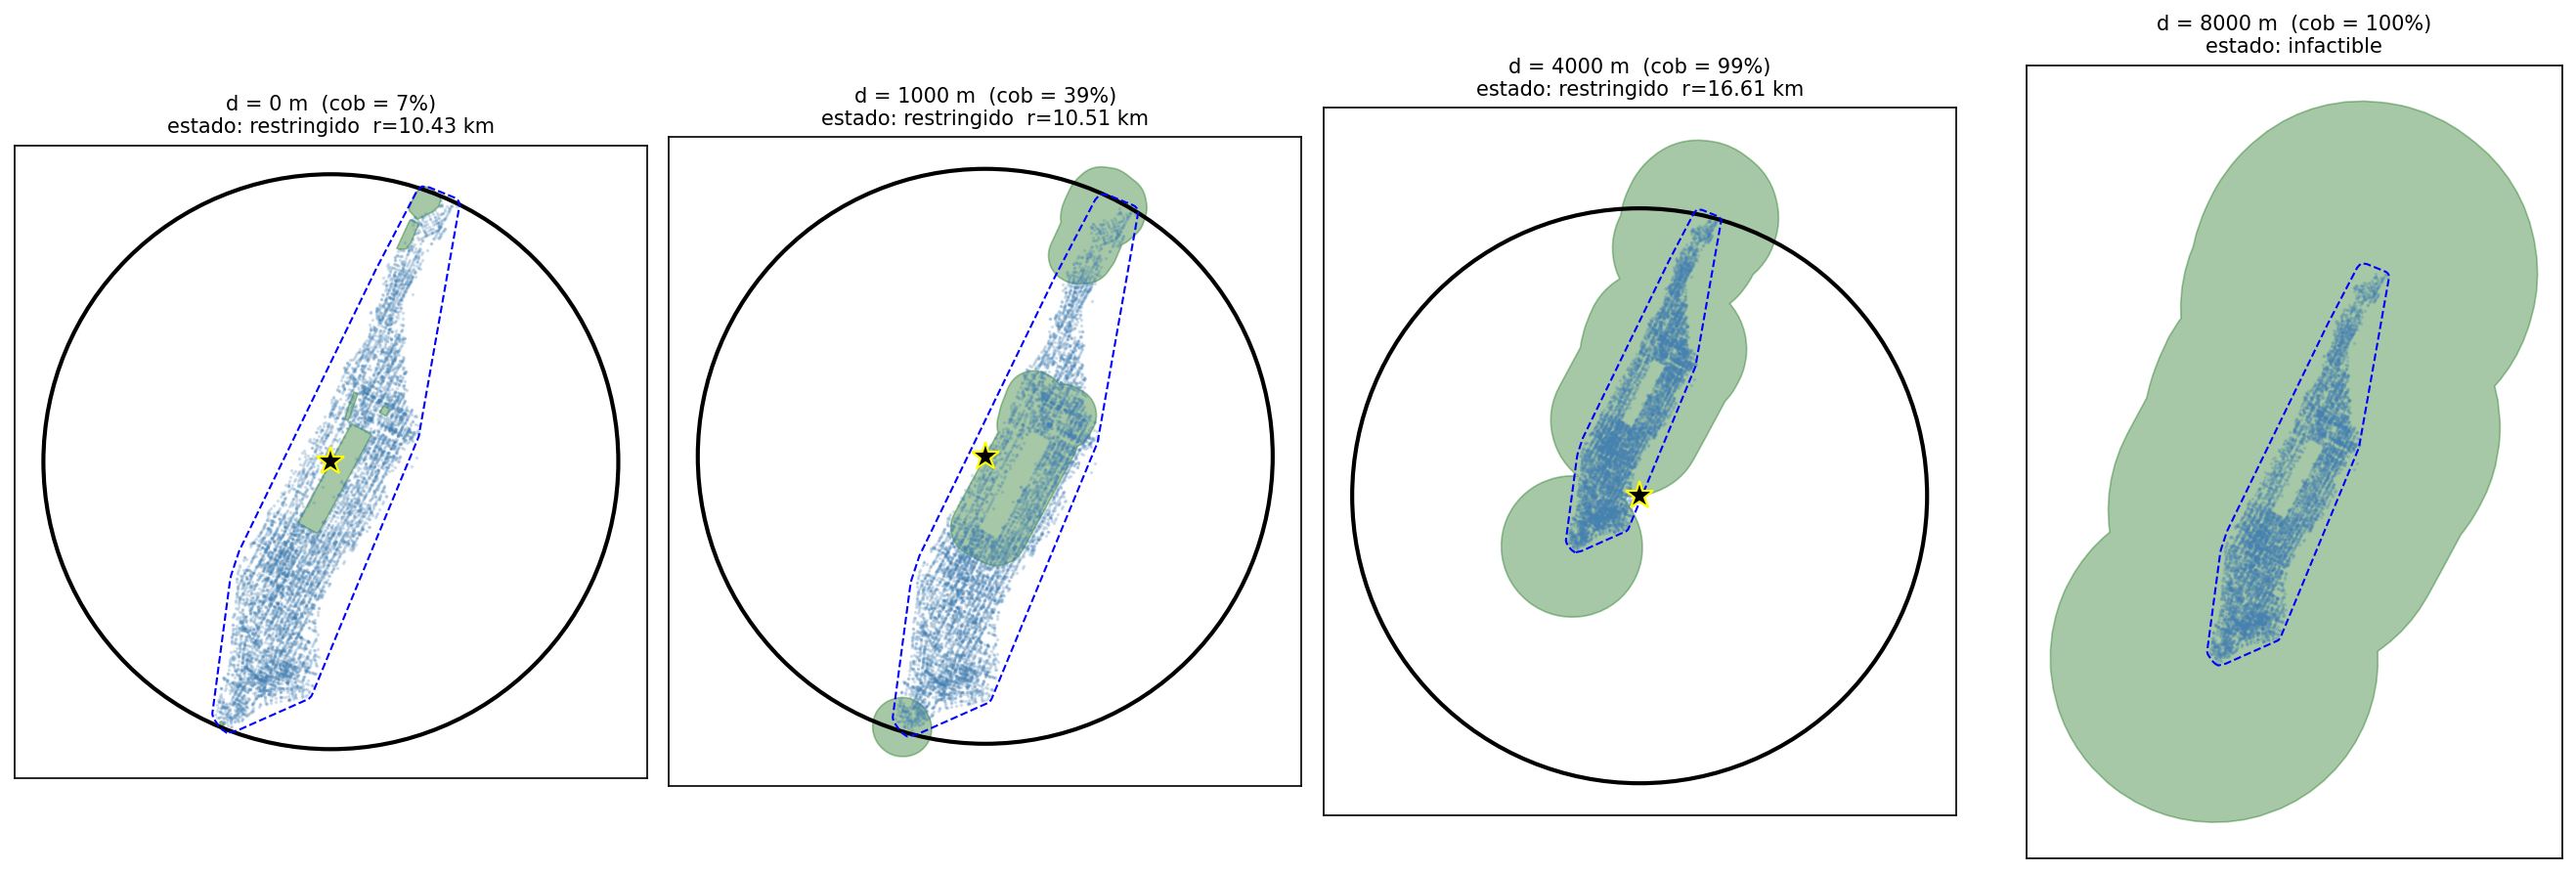
\includegraphics[width=\textwidth]{../results/figures/05_snapshots_buffer.png}
  \end{minipage}
  \caption{Experimento 3: condición de frontera.  Izq.: cobertura y radio
    vs.\ buffer.  Der.: cuatro snapshots con $d \in \{0, 1000, 4000, 8000\}$ m.
    La zona roja/naranja marca la transición a $\FF = \emptyset$.}
  \label{fig:frontera}
\end{figure}

\subsection{Experimento 4 (BONUS): Sensibilidad geométrica}
\label{sec:exp4}

Se evaluó el impacto de agregar zonas prohibidas de forma incremental, con
cuatro niveles de restricción:

\begin{enumerate}
  \item \textbf{Libre}: sin restricciones ($\FF = \RR^2$).
  \item \textbf{Solo Central Park}: $\FF = R \setminus Z_1$.
  \item \textbf{Barrera norte}: $\FF = R \setminus (Z_1 \cup Z_2 \cup Z_3)$.
  \item \textbf{Seis zonas}: $\FF = R \setminus \bigcup_{i=1}^6 Z_i$.
\end{enumerate}

Los resultados se muestran en la Tabla~\ref{tab:sens} y en la
Figura~\ref{fig:sens}.

\begin{table}[ht]
\centering
\caption{Sensibilidad geométrica: efecto de agregar zonas sobre la solución.}
\label{tab:sens}
\begin{tabular}{llrrrll}
\toprule
Nivel & \# Zonas & Radio (km) & $\Delta r$ (m) & $\Delta c$ (m) & Arista activa \\
\midrule
Libre            & 0 & 10.4244 & 0.00  & 0.0   & --- \\
Solo Central Park & 1 & 10.4293 & +4.93 & 320.5 & central\_park\#24 \\
Barrera Norte    & 3 & 10.4293 & +4.93 & 320.5 & central\_park\#24 \\
Seis zonas       & 6 & 10.4293 & +4.93 & 320.5 & central\_park\#24 \\
\bottomrule
\end{tabular}
\end{table}

El resultado es contundente: \textbf{solo Central Park es la restricción
vinculante (binding)}.  Agregar Morningside Park y Marcus Garvey (la
``barrera norte'') o las tres zonas restantes no cambia ni el centro ni el
radio.  La razón geométrica es que la dirección de mínimo radio conduce el
centro hacia el sur de Central Park (alejándose de las zonas del norte), por
lo que ninguna zona al norte llega a ser activa.

\begin{figure}[ht]
  \centering
  \begin{minipage}[b]{0.54\textwidth}
    \centering
    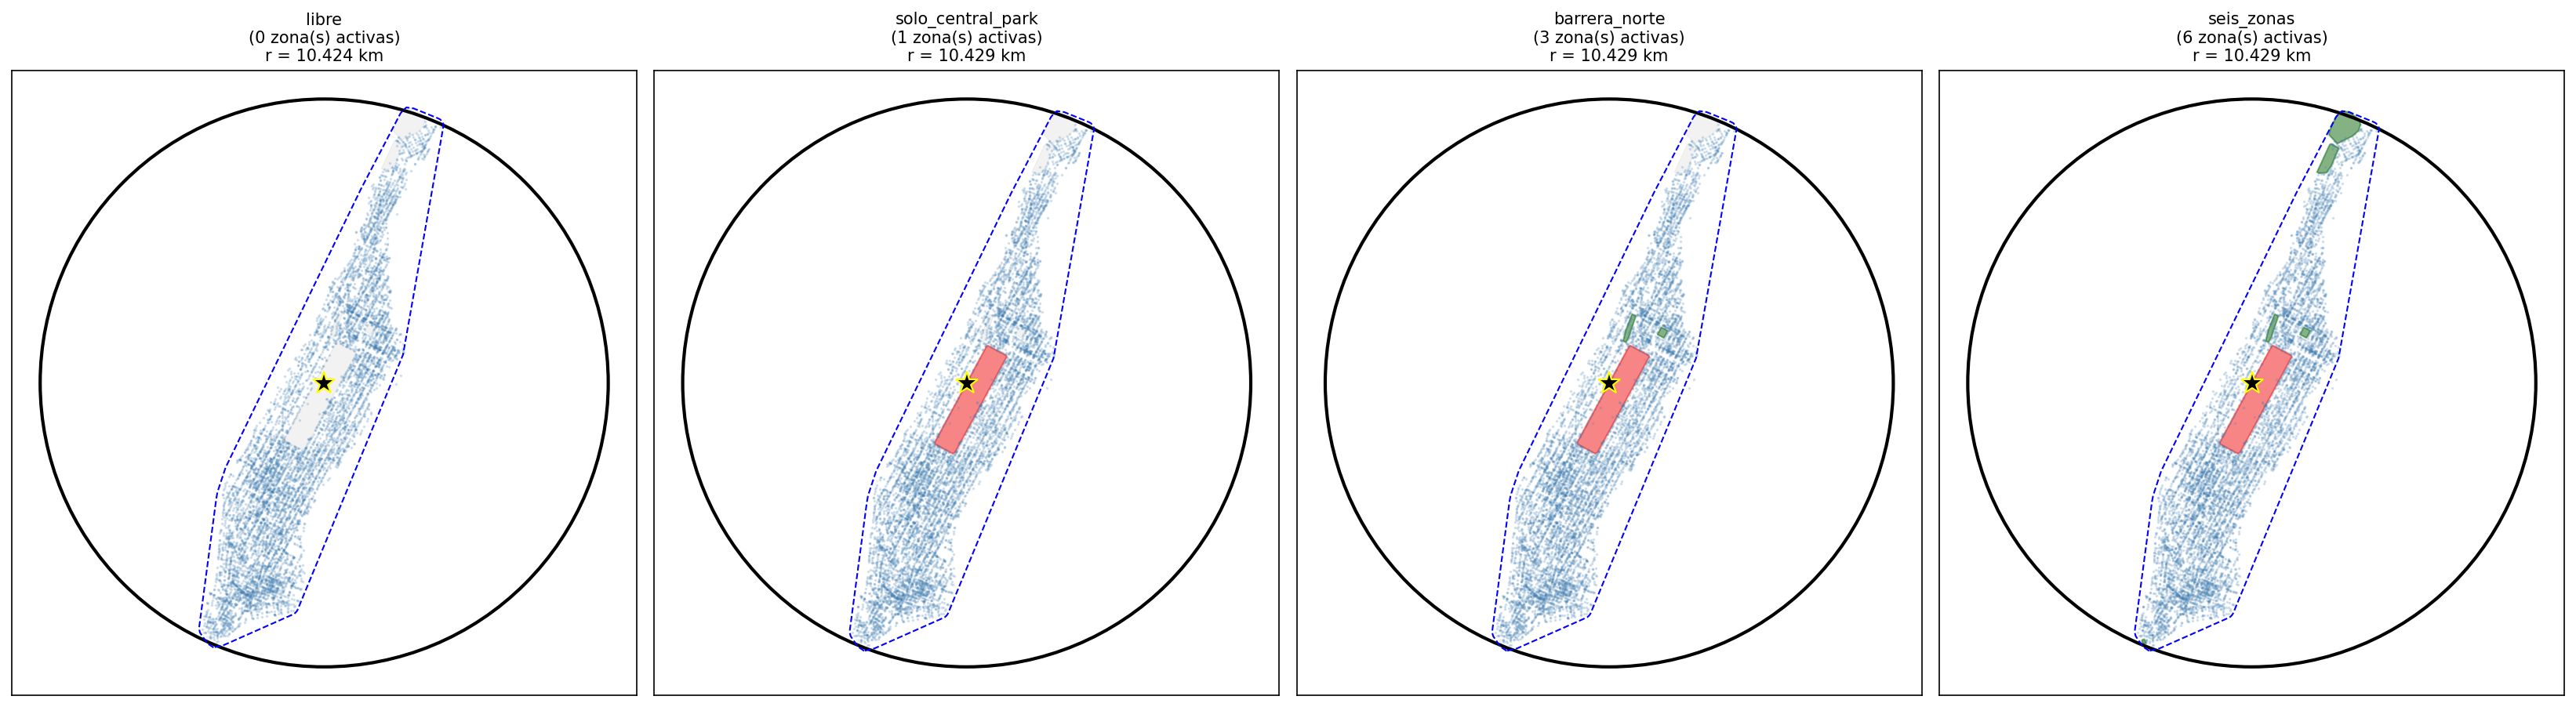
\includegraphics[width=\textwidth]{../results/figures/06_sensibilidad_niveles.png}
  \end{minipage}
  \hfill
  \begin{minipage}[b]{0.43\textwidth}
    \centering
    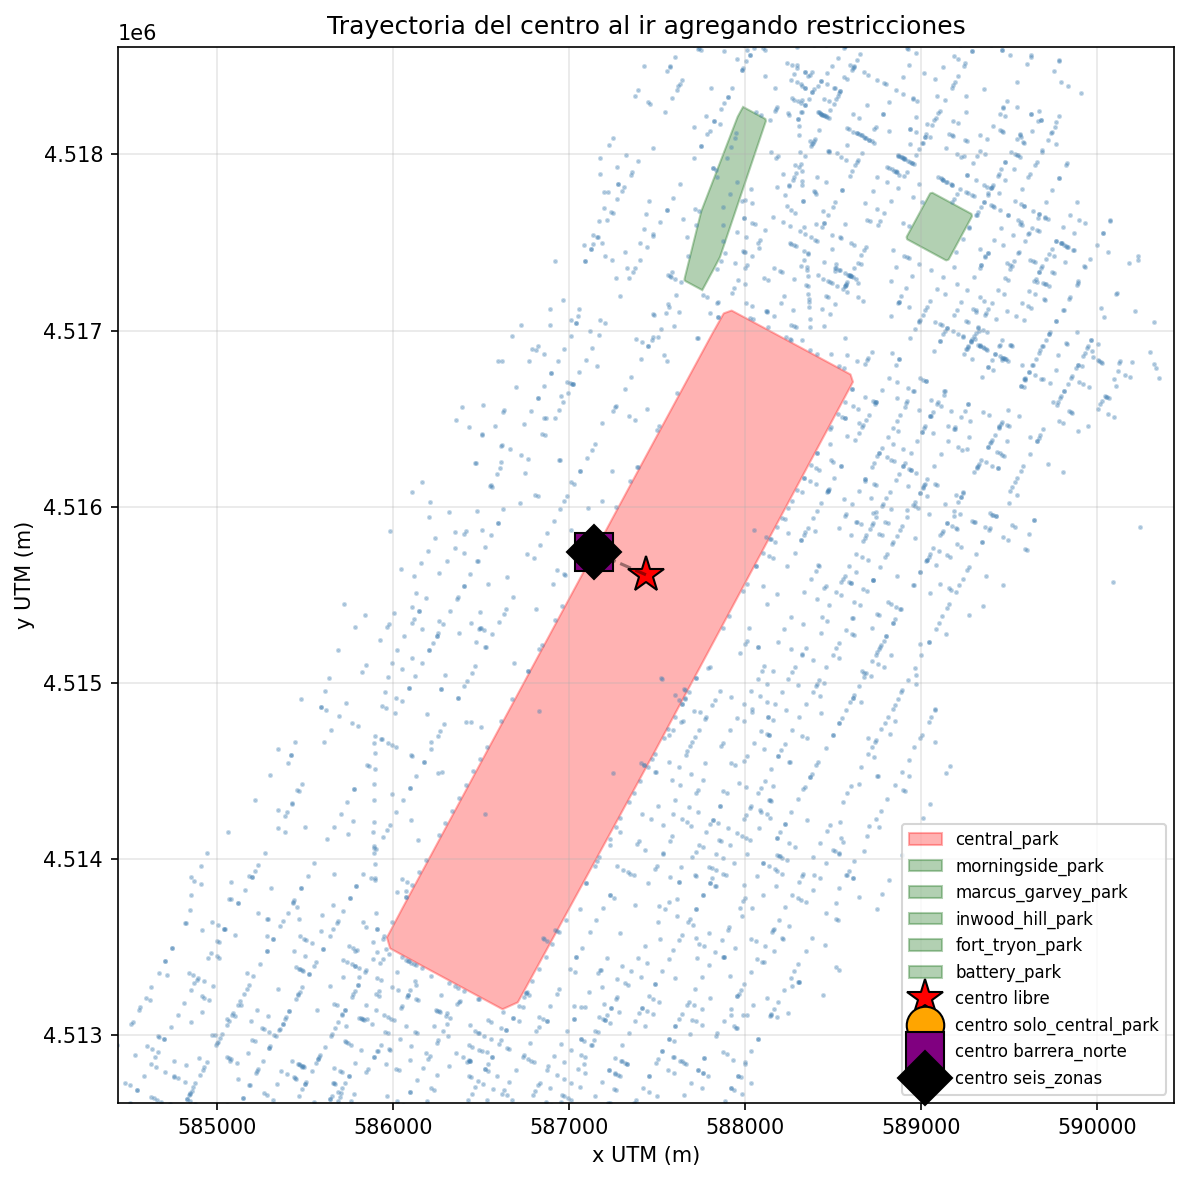
\includegraphics[width=\textwidth]{../results/figures/06_trayectoria_centro.png}
  \end{minipage}
  \caption{Experimento 4: sensibilidad geométrica.  Izq.: cuatro paneles,
    uno por nivel de restricción.  Der.: trayectoria del centro al agregar
    restricciones.  Los cuatro marcadores se superponen para los niveles 2--4,
    confirmando que solo Central Park es vinculante.}
  \label{fig:sens}
\end{figure}

% =============================================================================
\section{Implementación}
\label{sec:impl}

\subsection{Arquitectura del código}

El proyecto se estructura en módulos Python independientes dentro del
directorio \texttt{src/}:

\begin{table}[ht]
\centering
\caption{Módulos del proyecto.}
\label{tab:modulos}
\begin{tabular}{ll}
\toprule
\textbf{Módulo} & \textbf{Responsabilidad} \\
\midrule
\texttt{data\_loader.py}       & Descarga NYC Open Data; extracción de zonas OSM \\
\texttt{preprocessing.py}      & Limpieza, reproyección UTM, exportación Parquet \\
\texttt{seb\_primitivas.py}    & Bolas de 1, 2 y 3 puntos; test punto-en-bola \\
\texttt{seb\_seidel.py}        & Algoritmo de Seidel iterativo move-to-front \\
\texttt{seb\_welzl.py}         & Algoritmo de Welzl recursivo (baseline) \\
\texttt{validar\_seb.py}       & Verificación y comparación de bolas libres \\
\texttt{constraints.py}        & Semiplanos, tests en $F$, reproyección UTM \\
\texttt{seb\_restringido.py}   & SEB en segmento; enumeración de aristas activas \\
\texttt{validar\_seb\_restringido.py} & Validación SOCP con cvxpy \\
\texttt{app\_helpers.py}       & Conversiones UTM/WGS84; wrappers folium \\
\bottomrule
\end{tabular}
\end{table}

Los notebooks (01--06) ejercitan cada módulo sobre los datos reales y
producen las figuras almacenadas en \texttt{results/figures/}.

\subsection{Aplicación interactiva}

La aplicación \texttt{app.py} expone todos los experimentos en una interfaz
Streamlit con cuatro pestañas:

\begin{description}
  \item[Datos \& Mapa base.] Mapa folium con los accidentes clusterizados y
    las 6 zonas en gris.  KPIs: $n$ filtrado, radio libre, número de zonas
    y semiplanos.
  \item[SEB libre vs.\ restringido.] Toggles por zona, slider de buffer
    $d \in [0, 6\,000]$ m y botón ``Calcular''.  Muestra ambos círculos y
    los KPIs $\Delta r$, $\Delta c$, arista activa.  Si $\FF = \emptyset$,
    despliega un banner de advertencia.
  \item[Sensibilidad (Exp.\ 4).] Tabla de los 4 niveles (pre-calculada) y
    cuatro mini-mapas folium en grilla $2 \times 2$.
  \item[Frontera $\FF = \emptyset$ (Exp.\ 3).] Slider $d \in [0, 8\,000]$ m,
    mapa con zonas infladas e indicador de estado, más la curva de cobertura
    y radio pre-calculada.
\end{description}

Los filtros globales (año, hora, severidad, algoritmo) operan sobre el sidebar
y se aplican a todas las pestañas en tiempo real.

% =============================================================================
\section{Conclusiones}
\label{sec:conclusions}

\begin{enumerate}
  \item \textbf{El conjunto factible no-convexo no requiere métodos de
        optimización no-convexa global.}  La estructura LP-type del $\seb$ y
        la convexidad local de cada arista de $\partial\FF$ permiten resolver
        el problema exactamente en $O(E \cdot n)$ tiempo, donde $E = 260$ es
        el número de aristas de la frontera.

  \item \textbf{El centro libre cae en Central Park}, lo que hace necesario el
        modelo restringido para una ubicación logísticamente viable.  El
        desplazamiento de $\approx 320$ m al borde sur del parque impone una
        penalización de cobertura de apenas $0.047\%$ (+4.93 m sobre 10.4 km).

  \item \textbf{Solo la arista \#24 de Central Park es vinculante.}  Las otras
        cinco zonas prohibidas son geométricamente irrelevantes para este
        dataset: el óptimo se desplaza hacia el sur, lejos de las barreras
        del norte.  Esto ilustra que la \emph{estructura geográfica} del
        problema determina cuáles restricciones son activas.

  \item \textbf{Complejidad empírica $\approx O(n)$.}  La pendiente log-log
        del tiempo libre es $p = 0.942$ y la del restringido converge a 1
        para $n$ grande (confirmado hasta $n = 60\,000$).

  \item \textbf{Robustez ante infactibilidad.}  El algoritmo detecta
        $\FF = \emptyset$ sin lanzar excepciones y comunica el estado al
        llamante.  El buffer crítico está en $d^* \in (4\,438, 4\,469]$ m.

  \item \textbf{La representación por semiplanos es la piedra angular.}
        Transforma el test de pertenencia ``punto en polígono convexo'' en
        $k$ productos punto, permite detectar infactibilidad con cortocircuito,
        y es compatible con la vectorización numpy para los $O(E \cdot n)$
        evaluaciones de $f(t)$.
\end{enumerate}

% =============================================================================
\section*{Referencias}
\addcontentsline{toc}{section}{Referencias}

\begin{thebibliography}{9}

\bibitem{Seidel1991}
  Seidel, R. (1991).
  \textit{Small-dimensional linear programming and convex hulls made easy.}
  Discrete \& Computational Geometry, 6(3), 423--434.

\bibitem{Welzl1991}
  Welzl, E. (1991).
  \textit{Smallest enclosing disks (balls and ellipsoids).}
  En H. Maurer (ed.), \textit{New Results and New Trends in Computer Science},
  LNCS 555, pp.\ 359--370. Springer.

\bibitem{Megiddo1983}
  Megiddo, N. (1983).
  \textit{Linear-time algorithms for linear programming in $\mathbb{R}^3$
  and related problems.}
  SIAM Journal on Computing, 12(4), 759--776.

\bibitem{Sharir1992}
  Sharir, M., \& Welzl, E. (1992).
  \textit{A combinatorial bound for linear programming and related problems.}
  Proceedings STACS 1992, LNCS 577, pp.\ 567--579.

\bibitem{deBerg2000}
  de Berg, M., van Kreveld, M., Overmars, M., \& Schwarzkopf, O. (2000).
  \textit{Computational Geometry: Algorithms and Applications} (2nd ed.).
  Springer.

\bibitem{Fischer2003}
  Fischer, K., G{\"a}rtner, B., \& Kutz, M. (2003).
  \textit{Fast smallest-enclosing-ball computation in high dimensions.}
  ESA 2003, LNCS 2832, pp.\ 630--641.

\end{thebibliography}

\end{document}
